\chapter{Introduction\label{cha:chapter1}}

"Oder in the chaos and chaos in the order", is is how Osterhold \cite[p. 24f]{osterhold_2013} describes one of the two essential research directions of chaos theory. Furthermore she claims, "processes, procedures or structures that appear very disordered only prove to be chaotic prior to the point they are analyzed further". This generalized and theoretical approach can be directly transfered to computer science, especially the fields of information retrieval, data mining and data processing. 

\section{Motivation\label{sec:moti}}

The todays unbounded growth of information digitally available suggests a massive and chaotic collection of data. An in 2014 published report by ICD states that the digitalized data grow by 100\% every two years and will reach 44 zettabytes (10\textsuperscript{21} bytes) by 2020 - as many stars as known in the universe \cite{data_growth_2014}.
\\\\
Data in general, but also massive amounts of data, are only of value if they are utilized appropriately. Gaining deeper insights is the point of data transformation, data visualization or calculations on data. From a technical as well as an economical point of view a high degree of automation in data processing is required for maximizing the efficiency, especially when it comes to handling a high number of information entities \cite{labrinidis_jagadish_2012}. A large variety of software solutions is available that enable automated data processing for numerous domains and complexity levels. The solutions capture all levels of abstraction and reach from end user desktop applications, e.g. Microsoft Excel \cite{excel_2017} for the daily use, to low level software libraries, e.g. Pythons NumPy \cite{numpy_2017} for highly specialized research or industry applications. Electronic data processing boils down to applied mathematics and therefor relies on data of a deterministic structure. In computer science and mathematics there are well known specifications to transform and represent data in a computer understandable way. The canonical form \cite[p. 91 - 96]{dorst_doran_lasenby_2012}, database normalization \cite[p. 743]{halpin_tony_morgan_2010}or schema definitions \cite[p. 62]{halpin_tony_morgan_2010} are a selection of them. They are primary beneficial for generalizing data representation on different abstraction levels, for instance storing data in table-based format in files or specifying the order of bytes on hardware layer. A second evenly important aspect is the reduction of storage overhead when using predefined formats.
\\\\
Over the last 10 years specifications for data storage being as old as the computers itself find less and less supporters and therefor their compliance \cite{andlinger_2013}. Mainly to mention here are the database level and application level. Developments according to Moore's law \cite[p. 7ff, p. 87ff]{brock_2006} and constantly decreasing  costs of volatile memory are the enabler of that ongoing trend \cite{rhines_2016}.Computational power and high memory resources permit nowadays a by far more chaotic fashion of information storage. To perform analysis on data for reasonable time and resource costs in the past, it was essential to hold data in a well defined schema, i.e. the structure of the information entity with meta information about its attributes and types, and a unique storage format on file level. Modern data management solutions and databases loosened that strict demands tremendously. More available memory and higher computational resources are the enabler for heterogeneous data management. For instance, schema-less and document-oriented database management systems allow information entities with a deviating set of attributes to be stored \cite{hills_2016}. Data management and data retrieval systems even allow documents of different storage formats, e.g. PDF and text, to be maintained simultaneously. This trend mostly develops in the favor of the users on data producer side. Overhead on schema definitions, restrictions due to backward compatibility or synchronization of parties and stakeholders almost vanish. The new development is very well received in technical development and opens new challenges in different research areas.
\\\\
The drawbacks of that development have since been discovered by mostly consumers of such chaotic data \cite{lombardo_di_nitto_ardagna_2012}. Not only the contemporary style of handling and storing information has its disadvantages but also data which already come in a defined schema often do not fulfill the required granularity and purity. In certain data applications a high amount of manual work for quality assurance is invested \cite{wang_strong_1996}. Under the consideration of a rich landscape of different information entity formats data cleansing by hand, review by know-how owners or restructuration is applied. Data cleansing is the act of removing errors and solve inconsistencies in data to enhance their quality. This is only feasible on a manageable number of entities to be audited and becomes time and cost intense on big amounts of data. Initially claimed, that more powerful hardware resources even out the unsteady environment is only true if the the precision of the result must not meet a maximum. Instances exist in which a best possible outcome on data analysis is indispensable. Exposure to end consumers, mathematical analysis or unification of a broad number of data sources are case that demand the latter requirements to be met. 

\subsection{User exposure of data}

A primary important aspect with regard to the need of clean data is the exposure to end users, for example in web shops or desktop applications \cite{kim_niehm_2009}. To make a service resilient against competitors it is fundamental to satisfy the most valuable resource, the end users. The paying customer that often has a broad offer of similar services is most critical when it comes to functionality and appearance of the product \cite{huitfeldt_middleton_2001}. Insufficient information, unstructured layouts or poorly working features discourages customers quickly. Those shortcomings origin in underlying data problems. E.g. product filters of an online shop do not apply correctly if the data representation in the target attributes is not groomed appropriately or item characteristics are displayed in a inconsistent form when schemas do not match. The data diversity in this case derives from, inter alia, different sources, e.g. different supplies or partners in an online shop.

\subsection{Mathematical analysis} 

For analysis of messy data and calculation based on such 
very high requirements regarding granularity and purity exist. In theoretical mathematics well defined sets of inputs and possible outputs for functions, the definition of algebraic structures and the scopes of algebraic axioms, or the consistency of vector spaces are essential for applicability. This for example applies to techniques in the field of machine learning, especially to feature selection and feature engineering \cite{mitchell_1999}. Dimensions of feature vectors have to be assessed critically to avoid the curse of dimensionality\footnote{The curse of dimensionality describes among others a phenomena in high dimensional vector spaces where distances between each data sample become equal.} and control their sparsity. Sparse vectors hold little congruent information and are not well comparable. Considering only subsets of data that hold sufficient quality will effect results. For instance removing time windows due to certain quality filters change predictions on a time series as the continuity of data is not maintained.

\subsection{Unification of a broad number of data source} 

Use cases and applications exist where it is indispensable to combine information entities with varying structures originating from different sources. From a black-box point of view, a data aggregator only has one output format but must combine a range of input source formats. Not only different information providers cause a heterogeneous data, also the acquiring of the data plays a significant role. Facts like information storages and data warehouses grow over time while compromises on formats are made, technical and domain specifications for data management are not completely fulfilled, schemas vary, are underspecified or interpreted individually, impede a strict policy for homogeneous data. Information retrieval systems such as filter-engines, search-engines or recommendation systems face the stated problem. 
\\\\
Dasu and Johnson claim that 80\% of effort in data analysis is devoted to data preparation and feature engineering \cite{dasu_johnson_2003}. That number indicates a large potential for maximizing the overall gain in the field of data preparation. From the above addressed problems it can be seen that a large optimization leeway for automated data pre-processing exists. This space for optimization is considered as academic playground that motivates this work. Shifting the focus from data preparation to actual data utilization will be an enabler for quicker insight in data and lower the barrier for the development of data driven products.

\section{Objective and problem statement\label{sec:objective}}
The in the previous section outlined complex matters sketched the problems currently present. In a more generalized aspect it can be claimed, that neither data from normalized sources, and even less data from schema-less sources often fulfill the required granularity and purity for above mentioned use cases. The novel amount of data digitally available and the innovative desire of data driven product development often conflicts in the quality of the underlying resource. A gap emerges that is most often directly linked to additional manual effort. This gap appears in different data formats, as well as in the semantic of data. In different systems wordings of characteristics vary and therefor can not be directly related. Furthermore invalid data, misspellings and missing information, coming from manual data entry, impede and bias analyses. This thesis concerns stated data quality issues and describes an solution to overcome the problems of diversity of available digital data.  

\section{Scope and target\label{sec:scope}}
The target of this work is to analyze the current state of heterogeneous data as outlined in the previous section. This analysis is discussed and assessed. In a problem driven approach the findings are split into sub problems and key points with large optimization potential are identified. Those key points are investigated on deeper and an overview of available techniques, technologies and approaches from different fields of computer science to tackle the state problems is provided.
\\\\
The main emphasis of this work is on the automation of preparation steps. Those are combined within a framework that enables feature extraction from semi-structured data. The key asset to be reduced with the proposed framework is manual overhead on data preparation. Equally important is the extendability and adaptability of the tool set towards unseen data and temporal changes in data. Concepts for a administration application in regards to quality assurance and framework maintainability are given. Those concepts are designed such that the remaining manual work can be reduced. 

A second focus lies on the adaptability to an changing environment. Predefined and agreed constrains and schemas do not last forever. A violation of that rule set does not necessarily mean corrupt data. Under a different definition such data are in fact correct. This rises the need for a framework that adapts to the input data over time. Possible solutions can be taken from the field of machine learning as well as database management systems. Updating a learned models or collected data in an iterative approach is considered as promising. 
\\\\
On a less abstract level this work addresses the stated problems in the domain of food recipes. Here, the recipe is considered as information entity that comes in various semi-structured forms containing, among other attributes, a set of ingredients. The ingredients itself are combinations of a  set of attributes that have a vast number of manifestations as well as non-deterministic order. References and similarities to other domains, e.g. product catalogs, are drawn and highlighted to proof the generalization ability of the proposed framework. A conclusion will assess the feasibility of such a system, review the performance result as well as address shortcomings.
\\\\
The overall target is to find a framework based solution that provides a tool set for extraction automation of essential key features from unequal information entities. As illustrated below the outcomes of this work can be adopted in applications that require high quality data. Figure \ref{fig:framework-sketch} shows the proposed framework as part of a recommendation system utilized by 3rd party data.
\\
\begin{figure}[htb]
  \centering
  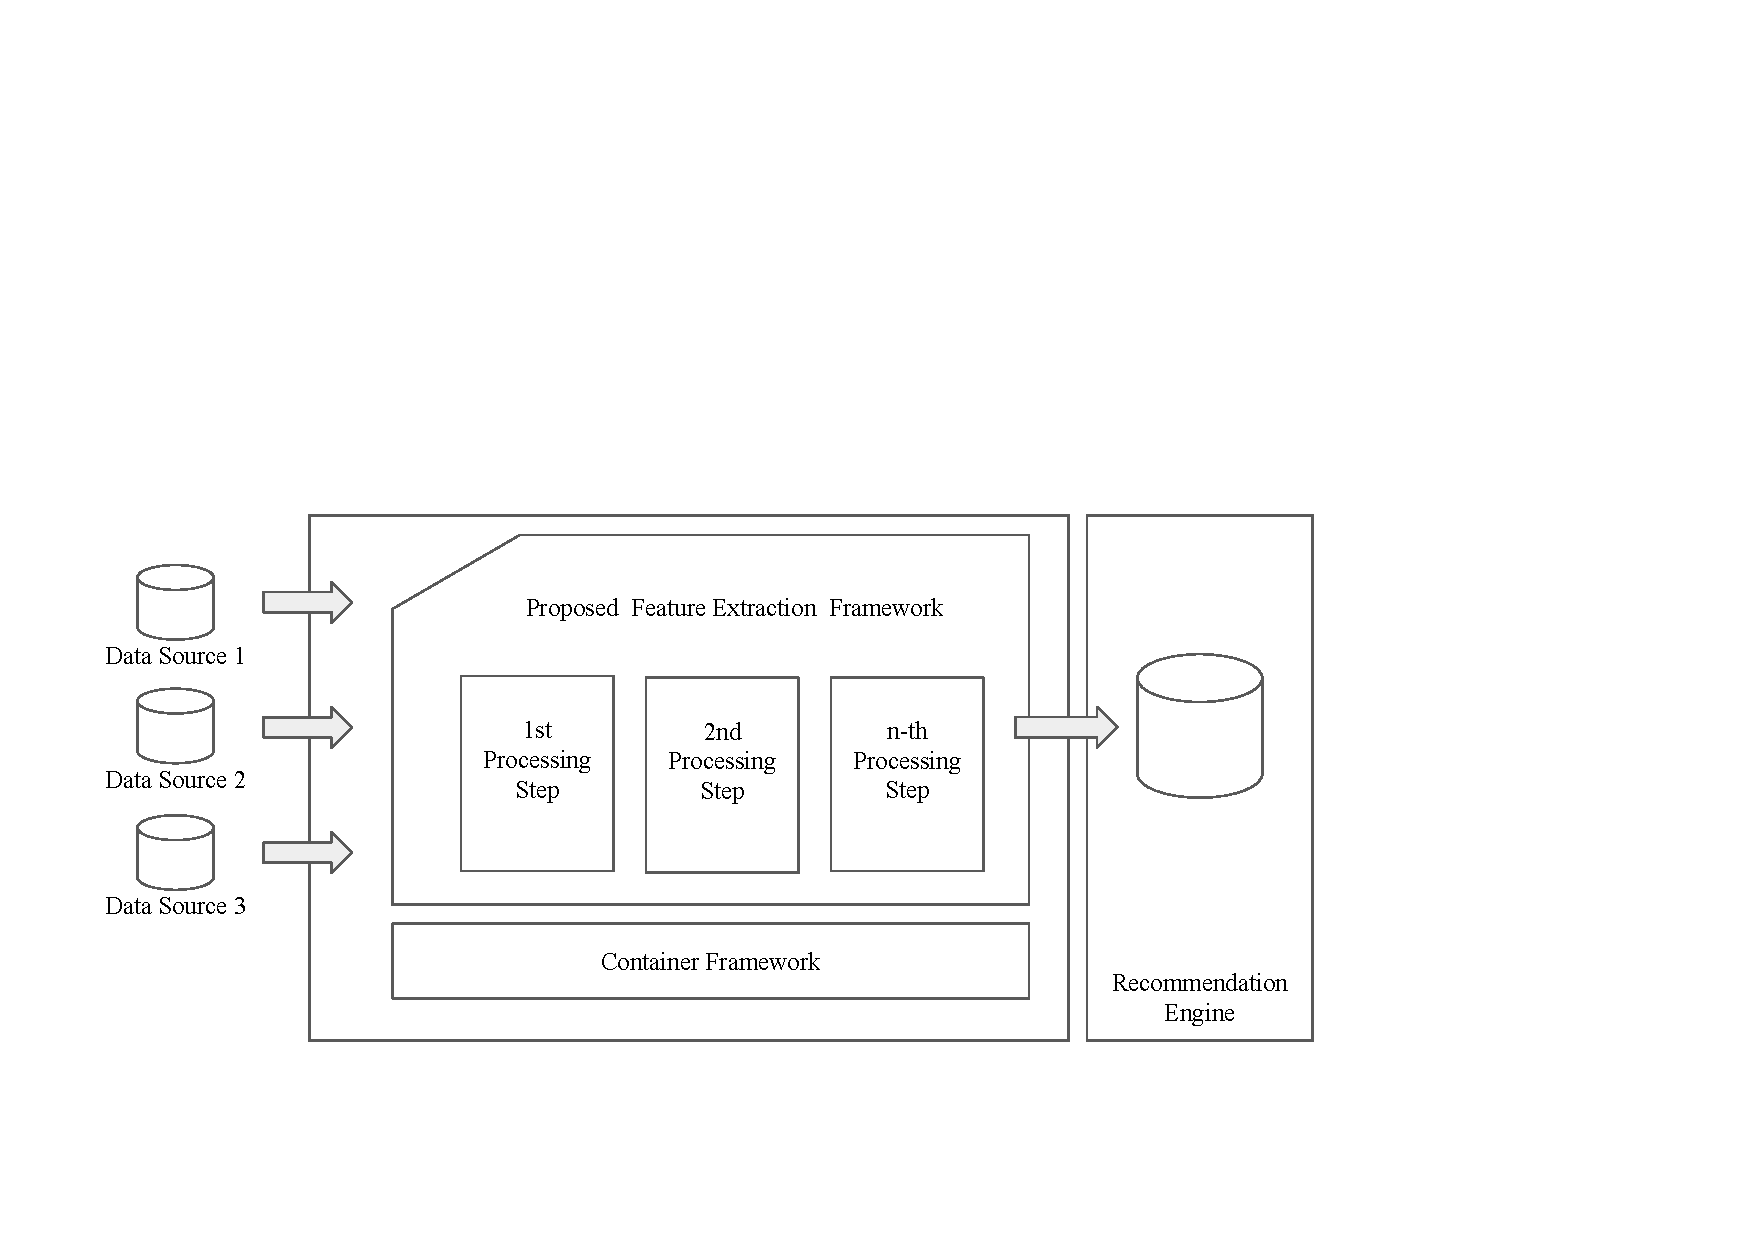
\includegraphics[width=0.9\textwidth]{framework-sketch}\\
  \caption{Feature extraction framework}\label{fig:framework-sketch}
\end{figure}

\section{Outline\label{sec:outline}}

In this section we well have a short overview of the chapters in this thesis. This work is separated into 7 chapters.
\\\\
\textbf{Chapter \ref{cha:chapter2}} covers aspects about fundamentals. As state above the thesis follows a problem driven approach, therefor the underlying structure and problems of modern data storage concepts are analyzed, broken down in subproblems and finally assessed.
\\\\
\textbf{Chapter \ref{cha:chapter3}} uses the findings of chapter \ref{cha:chapter2} and develops requirements on the proposed framework. An additional explanation of each individual requirement is given to demonstrate its necessity.
\\\\
\textbf{Chapter \ref{cha:chapter4}} uses the specifications and requirements from chapter \ref{cha:chapter3} and elaborates in a top down approach a concept for an automated framework for feature extraction. Different aspects regarding the problems of chapter \ref{cha:chapter2} are covered and abstract solutions and concepts are introduced. The overall concept aims for a subsequent reference implementation of the suggested framework.
\\\\
\textbf{Chapter \ref{cha:chapter5}} describes the implementation of the suggested framework. A research on underlying technologies, the choice of a implementation language as well as structural decisions are conducted. Components on different layers are explained and applied patterns discussed. 
\\\\
\textbf{Chapter \ref{cha:chapter6}} interprets the findings and outcomes of the precedent three chapters. The discussion of the applicability of the proposed framework is lead under the aspect of the reference implementation. The concepts are challenged and cross-checked for their feasibility under a technical perspective.
\\\\
\textbf{Chapter \ref{cha:chapter7}} summarizes the thesis, describes the problems that occurred and gives an outlook about future work.